\chapter{联邦学习的安全混洗模型}
\label{ch4}
\section{引言}
上一章节中所提出的本地自适应差分隐私方案是通过在客户端将梯度上传至参数服务器前,对梯度添加自适应噪声,尽管方案采用了本地差分技术减少一定程度的隐私预算,但不可避免的会降低联邦学习模型的准确性以及学习效率。正如\upcite{ref37}所指出的,一个复杂的隐私保护系统将多个本地差分隐私的算法进行组合,从而导致这些算法的隐私成本增长。也就是说,隐私预算为ε1和ε2的局部差异化算法的组合会消耗的隐私预算总和为ε1+ε2。使用联邦学习训练的联合模型需要客户在多次迭代中向中央服务器上传梯度更新。如果在迭代训练过程中的每一次迭代都应用本地自适应差分隐私,隐私预算就会累积起来,从而导致总隐私预算的爆炸。现有的本地差分隐私协议对于多维聚集的联邦学习框架可能是不可行的,局部噪声带来的误差会随着维度系数的增加而加剧\upcite{ref38},从而大大降低模型的精度。而且,当参与一次迭代的客户端数量达到上千人时,会导致聚合任务升级成一个高维任务,隐私预算暴增。
而且,值得关注的是,不同的用户有不同的隐私需求,不同的用户上传的梯度对于联合模型的贡献比也有差异,因此本章将提出混合差分隐私技术,构造一个全新的可信第三方——混洗器,与本地差分隐私相结合,实现的方案能提高全局模型的精度,也保证在更低的隐私成本下达到相同的隐私预算。

在本章节中我们提出了一个在联邦学习中的安全混洗器,本地客户端使用自适应差分隐私对于模型的输出进行加躁,然后安全混洗器从客户端上传的样本中随机采样,将收集到的梯度以维度进行拆分,打乱次序,达到隐私放大效果,再采用梯度稀疏化的技术筛选对联合模型贡献较高的梯度,发送给中央服务器进行聚合。安全混洗器作为一个可信第三方,独立于服务器并专门用于本地客户端梯度的子采样、混洗、上传。这个模型通过子采样和混洗两者的结合达到隐私放大效应,从而提高了整体联邦学习模型的精度。当本地差分隐私添加更少的噪音时,对于同样的中央服务器能达到相同水平的隐私预算。

我们将在本章节详细的描述该框架中各个模块的设计和实现过程。

\section{安全混洗模型}
如图\ref{fig:联邦学习中的安全模型框架}所示,该框架主要由本地客户端、混洗器和中央服务器3部分组成:
\begin{itemize}
  \item 本地客户端: 基于第三章的本地自适应差分隐私方案,在模型训练的梯度下降算法中对梯度进行自适应的扰动,得到满足$\left(\epsilon_{c}+\epsilon_{l}\right)$差分隐私的梯度。
  \item 混洗器: 一个半诚信的第三方。首先动态采样本地客户端上传的梯度,然后借助现有的安全混洗协议在对数据一无所知的情况下,对子采样后的梯度完成安全的拆分混洗操作,通过隐私放大效应使得算法满足$\epsilon_{0}$-差分隐私,达到梯度匿名机制,最后将混洗后的结果发送至中央服务器。
  \item 中央服务器: 一个诚实但好奇的第三方。服务器接受混洗器上传的梯度并进行聚合,然后更新全局模型。
\end{itemize}

假设现在有m个本地客户端,每个客户端表示为$i \in[m]$,有本地数据集\\$\mathcal{D}_{i}=\left\{d_{i 1}, \ldots, d_{i r}\right\} \in \mathbb{S}^{r}$,由$r$ 个数据集合构成。$F_{i}(\theta)$表示在客户端$i$的本地数据集 $\mathcal{D}_{i}$上进行训练,对于模型梯度$\theta \in \mathbb{R}^{d}$进行衡量的损失函数,其中$F_{i}(\theta)=\frac{1}{r} \sum_{j=1}^{r} f\left(\theta ; d_{i j}\right)$,$f(\theta ; \cdot): \mathcal{C} \rightarrow \mathbb{R}$是凸函数。中央服务器的目标是找到一个最佳的模型参数向量$\theta^{*} \in \mathcal{C}$ 使得损失函数$\min _{\theta \in \mathcal{C}}\left(F(\theta)=\frac{1}{m} \sum_{i=1}^{m} F_{i}(\theta)\right)$最小,其中隐私性满足单个客户端的隐私预算,也就是满足$\epsilon_{0}$-LDP。在算法\ref{联邦学习中的安全模型算法}中,首先我们从m个客户端中随机挑选k个客户端,表示为集合$\mathcal{U}_{t}$,其中$k \leq m$。每个客户端$i \in \mathcal{U}_{t}$从本地数据集中抽样$\mathcal{S}_{i t}$个样本训练模型,计算梯度$\nabla_{\theta_{t}} f\left(\theta_{t} ; d_{i j}\right)$。第$i$个客户端采用基于第三章的自适应本地差分隐私方案,添加噪声、裁剪梯度,然后将梯度发送给混洗器。混洗器对收到的梯度进行拆分混洗,然后发送给中央服务器。最后,中央服务器对混洗后的梯度进行聚合求均值,更新全局模型。

\begin{algorithm}[!htb]
	\caption{联邦学习中的安全模型算法:$\mathcal{A}_{\text {csdp}}$}
	\label{联邦学习中的安全模型算法}
	\begin{algorithmic}[1]
		\footnotesize
		\STATE \textbf{输入:} 数据集$\mathcal{D} \quad=\bigcup_{i \in[m]} \mathcal{D}_{i}$, $\mathcal{D}_{i}=\left\{d_{i 1}, \ldots, d_{i r}\right\}$, loss function $F(\theta)=$ $\frac{1}{m r} \sum_{i=1}^{m} \sum_{j=1}^{r} f\left(\theta ; d_{i j}\right)$,本地差分隐私预算$\epsilon_{0}$,梯度范数阈值$C$,模型学习率$\eta_{t}$
		\STATE \textbf{初始化:} $\theta_{0} \in \mathcal{C}$
		\FOR{$t \in[T]$}
			\STATE \textbf{客户端采样:} 混洗器从k个客户端中随机采样$i \in \mathcal{U}_{t}$个客户端
			\FOR{客户端$i \in \mathcal{U}_{t}$}
				\STATE \textbf{梯度选择:} 客户端i从s个样本空间中随机采样$\mathcal{S}_{i t}$个梯度
				\FOR{样本$j \in \mathcal{S}_{i t}$}
					\STATE $\mathbf{g}_{t}\left(d_{i j}\right) \leftarrow \nabla_{\theta_{t}} f\left(\theta_{t} ; d_{i j}\right)$
					\STATE ${\mathbf{g}}_{t}\left(d_{i j}\right) \leftarrow \mathbf{g}_{t}\left(d_{i j}\right) / \max \left\{1, \frac{\left\|\mathbf{g}_{t}\left(d_{i j}\right)\right\|_{p}}{C}\right\}^{3}$
					\STATE $\mathbf{q}_{t}\left(d_{i j}\right) \leftarrow \mathcal{R}_{p}\left(\tilde{\mathbf{g}}_{t}\left(d_{i j}\right)\right)$
				\ENDFOR
				\STATE 客户端i将$\left\{\mathbf{q}_{t}\left(d_{i j}\right)\right\}_{j \in \mathcal{S}_{i t}}$发送给混洗器
			\ENDFOR
			\STATE \textbf{混洗器:} 混洗器对于$\left\{\boldsymbol{q}_{t}\left(d_{i j}\right): i \in \mathcal{U}_{t}, j \in \mathcal{S}_{i t}\right\}$中的权重进行拆分混洗,然后上传给中央服务器
			\STATE \textbf{中央服务器聚合梯度:}$\overline{\mathbf{g}}_{t} \leftarrow \frac{1}{k s} \sum_{i \in \mathcal{U}_{t}, j \in \mathcal{S}_{i t}} \boldsymbol{q}_{t}\left(d_{i j}\right)$
			\STATE \textbf{梯度下降:}$\theta_{t+1} \leftarrow \prod_{\mathcal{C}}\left(\theta_{t}-\eta_{t} \overline{\mathbf{g}}_{t}\right)$
		\ENDFOR
		\STATE \textbf{输出:}最终全局模型参数$\theta_{T}$

	\end{algorithmic}
\end{algorithm}

\begin{figure}[!hbt]
\centering
	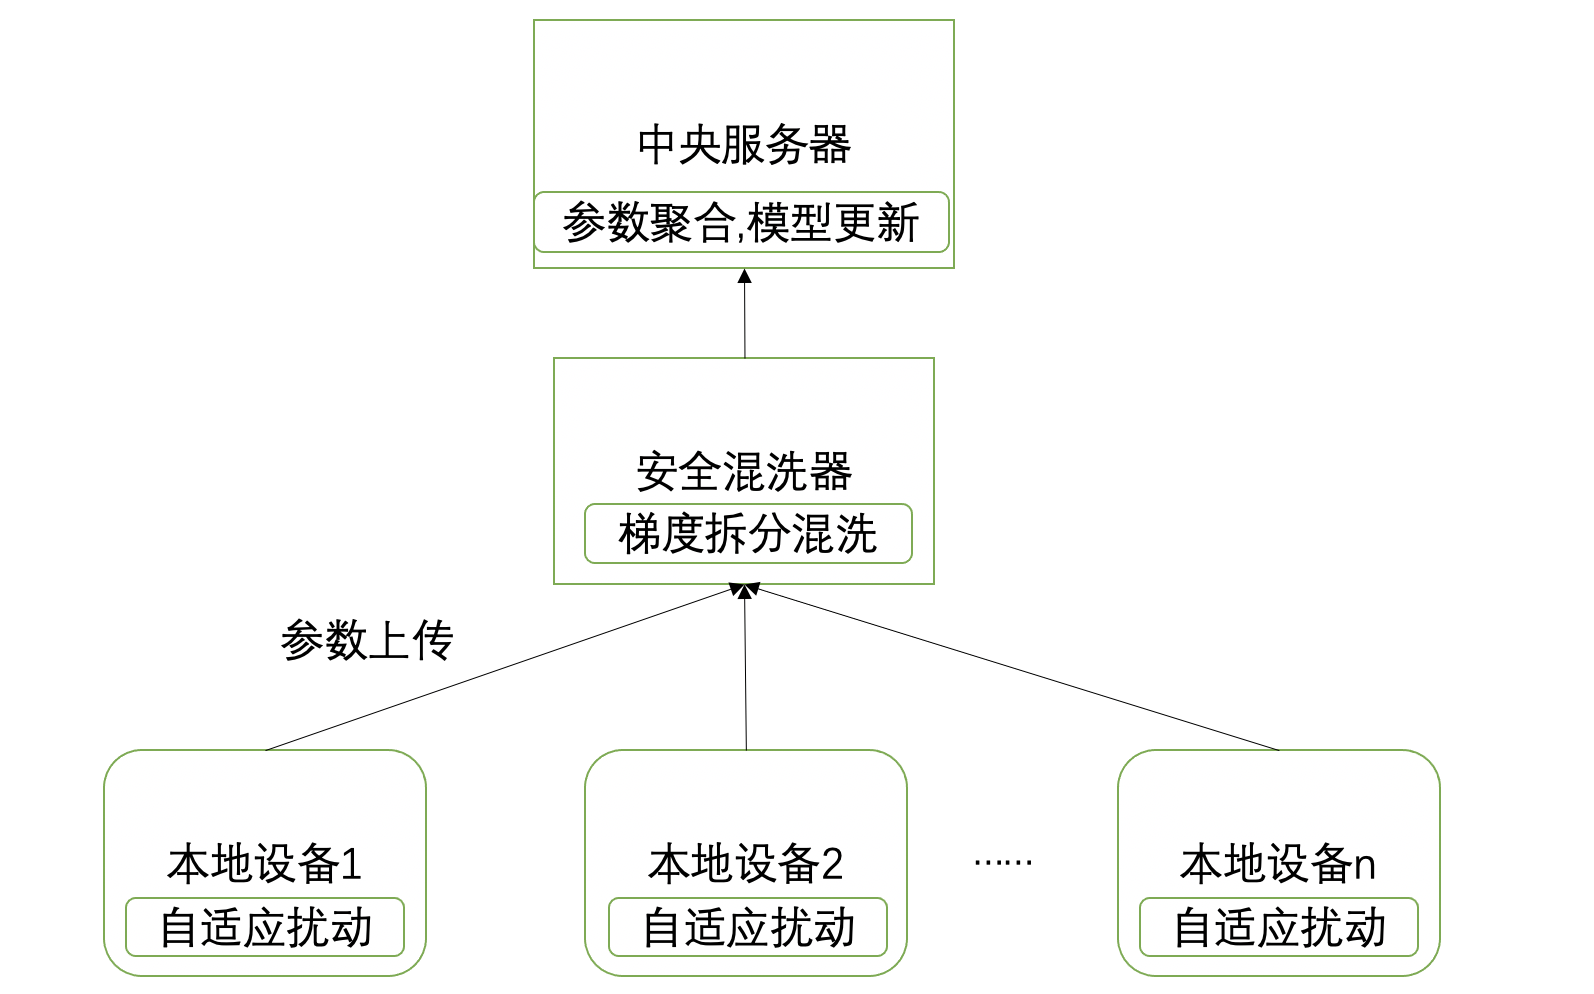
\includegraphics[scale=0.5]{fig2/C4/shuffle模型}%联邦学习的系统架构
	\caption{联邦学习中的安全模型框架}
	\label{fig:联邦学习中的安全模型框架}	
\end{figure}

\subsection{客户端抽样}
假设在空间$\mathcal{U}$中我们有一个数据集$\mathcal{D}^{\prime}=\left\{U_{1}, \ldots, U_{r_{1}}\right\} \in \mathcal{U}^{r_{1}}$,其中包含$r_{1}$个样本元素。如定义\ref{子采样}所示,本文定义一个子采样程序:首先采样一个客户端数据集$\mathcal{D}^{\prime} \in \mathcal{U}^{r_{1}}$,再从中采样一个子集作为客户端的本地训练数据。
\begin{define}[子采样]\label{子采样}
定义一个抽样程序$\operatorname{samp}_{r_{1}, r_{2}}: \mathcal{U}^{r_{1}} \rightarrow \mathcal{U}^{r_{2}}$,其中$r_{2} \leq r_{1}$:从输入的数据集$\mathcal{D}^{\prime} \in \mathcal{U}^{r_{1}}$ 中以随机概率抽选一个子数据集$\mathcal{D}^{\prime \prime}$,数据集$\mathcal{D}^{\prime}$中的每个元素在数据集$\mathcal{D}^{\prime \prime}$中出现的概率为$q=\frac{r_{2}}{r_{1}}$。
\end{define}

\subsection{混洗器}
先前的研究工作(H Brendan McMahan, Daniel Ra- mage, Kunal Talwar, and Li Zhang. Learning differen- tially private recurrent language models. arXiv preprint arXiv:1710.06963, 2017.)表明,在联邦学习模型中,假如在某个时间段数据是被适当的匿名化,并将数据之间的耦合信息拆分后,模型整体的隐私保障可以得到极大的改善。在第三章中的隐私保护方案是基于本地客户端训练数据的,而面对恶意的中央服务器甚至是恶意的第三方攻击者时,无法保障每个客户端的隐私。

因此在本章中,我们针对客户端上传的梯度,进行参数的拆分混洗,通过混洗器达到客户端的匿名性,打破从中央服务器接收的数据与特定客户端之间的联系,并在每次迭代中从同一客户端发送的梯度更新中将信息解耦。

客户端的匿名性可以通过现有的多种机制来实现,这取决于中央服务器在特定场景下如何跟踪客户端。作为一个典型的保护隐私的最佳做法,每个客户对服务器有一定程度的匿名性,以使客户的个人身份识别与他们的权重更新无法关联。例如,如果服务器通过IP地址追踪客户,每个客户可以通过使用网络代理、VPN服务[Belesi, 2016]、公共WiFi接入[Dingledine等人,2004]产生一个无法追踪的IP地址。再比如,如果服务器通过软件生成的元数据(如ID)来追踪客户,每个客户可以在向服务器发送元数据之前将其随机化。

但是,我们认为,客户端的匿名性不足以防止通信链道的攻击。例如,如果客户端在每次迭代中同时上传了大量的权重更新,中央服务器仍然可以将它们连接在一起。因此,我们设计了混洗器,以打破来自相同客户的模型权重更新之间的联系,并将其放置于客户端上传梯度更新至中央服务器之间,使中央服务器更难结合多个客户端的同步更新来推断任何客户的更多信息。

如下图所示,我们的混洗器通过以下步骤对客户端上传的梯度参数进行混洗,然后上传给中央服务器:
\begin{itemize}
	\item 权重分割:每个客户端都对其本地模型的权重进行分割,但给每个分割后的元素贴上一个id,以表明其在网络结构中的权重位置。
	\item 权重混洗:对于所有客户端分割后的权重采用随机扰动机制进行混洗。
\end{itemize}

\begin{figure}[!hbt]
\centering
	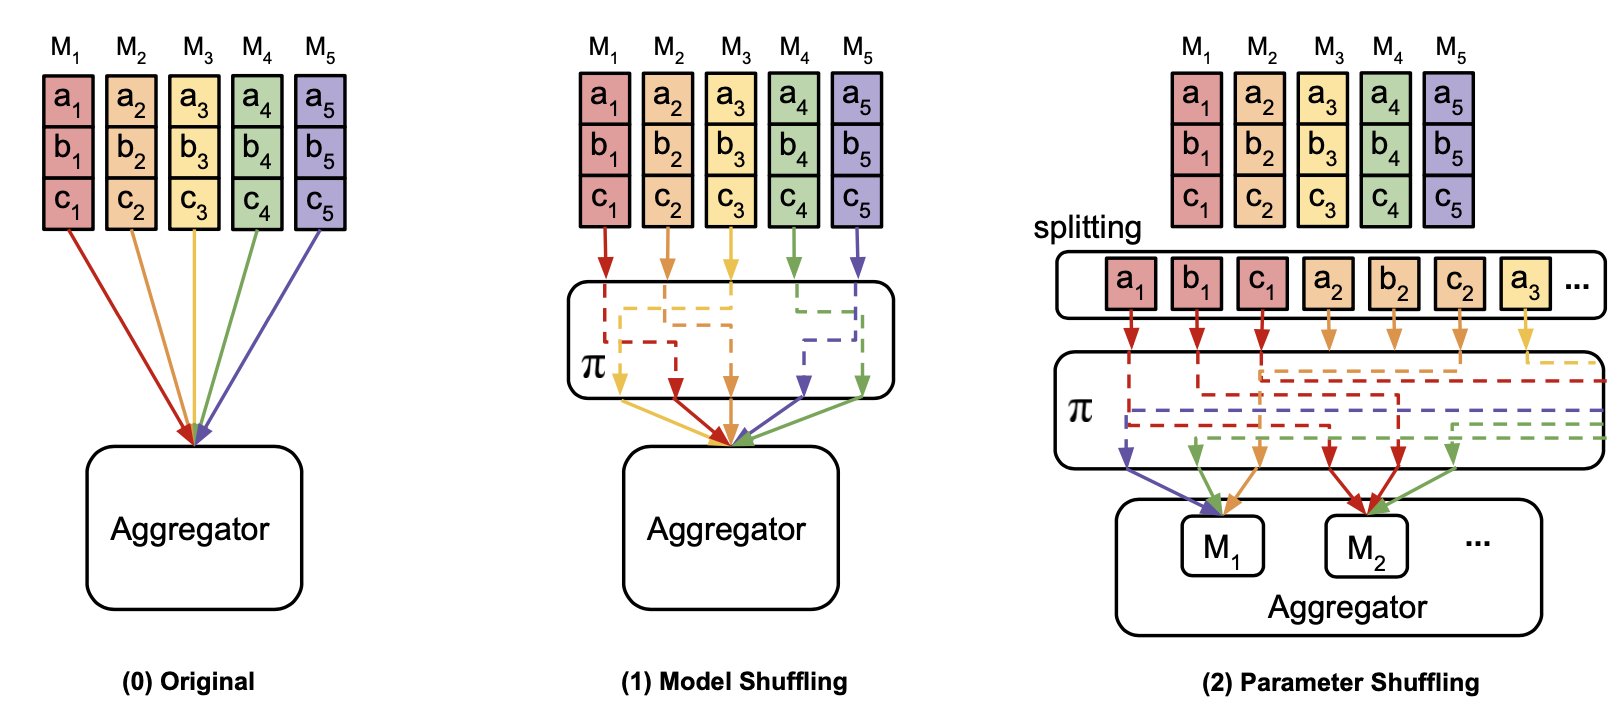
\includegraphics[scale=0.4]{fig2/C4/混洗器}%联邦学习的系统架构
	\caption{联邦学习安全模型中执行参数拆分混洗的混洗器}
	\label{fig:联邦学习安全模型中执行参数拆分混洗的混洗器}	
\end{figure}

\begin{algorithm}[!htb]
	\caption{混洗器中的拆分混洗算法}
	\label{混洗器中的拆分混洗算法}
	\begin{algorithmic}[1]
		\footnotesize
		\STATE \textbf{Input:} 本地客户端添加自适应扰动后的权重$W_{l+1}^{s}$
	    \STATE 对权重$W_{l+1}^{s}$进行分割,给每个元素分配id
	    \FOR{$w^{s} \in W$}
	    \STATE 用一个唯一的id标记元素的位置
	    \STATE 在通信时刻(0,$T$)期间随机采样$t_{i d}^{s} \leftarrow U(0, T) \%$
	    \ENDFOR
	    \STATE 在时刻 $t_{i d}^{s}$将梯度$(i d, w_{i d})$发送给中央服务器
	\end{algorithmic}
\end{algorithm}


\section{隐私放大效应}
隐私放大(privacy amplification)是本章所提出的安全框架中混洗器对隐私效果增强的理论分析,基于该理论,可将现有的本地化差分隐私方法直接应用在安全框架上。

在算法\ref{联邦学习中的安全模型算法}中,每个本地客户端采用第三章的满足$\left(\epsilon_{c}+\epsilon_{l}\right)$的自适应本地差分隐私算法,将参数上传至混洗器进行拆分混洗后,所获取的数据满足 $\varepsilon_{\mathrm{c}}-\mathrm{DP}$。从 $\left(\epsilon_{c}+\epsilon_{l}\right)$到 $\varepsilon_{\mathrm{c}}$ 的转变可通过隐私放大理论证明。$\left(\epsilon_{c}+\epsilon_{l}\right)$ 对应于较大的数值, 表示较低的隐私性; $\varepsilon_{\mathrm{c}}$ 对应于较小的数值, 表示较高的隐私性。因此经过混洗器后,隐私性得到了增强。由差分隐私的强组合性可保证算法$\mathcal{A}_{\text {csdp}}$在每次迭代中对每个样本$d_{i j}$都能保证$\epsilon_{0}$的本地差异隐私。因此本节只需要分析采样和混洗操作的隐私放大性。

\begin{theorem}\label{隐私性证明}
算法\ref{联邦学习中的安全模型算法}是满足$(\epsilon, \delta)-$差分隐私的,当对于任意$\delta$,$\delta>0$ ,并且有:
$$
\epsilon=\mathcal{O}\left(\epsilon_{0} \sqrt{\frac{q T \log (2 q T / \delta) \log (2 / \delta)}{n}}\right)
$$
\end{theorem}

假设在联邦学习模型中,需要迭代的次数为$t \in[T]$。$\mathcal{M}_{t}\left(\theta_{t}, \mathcal{D}\right)$表示在时刻$t$对于数据集$\mathcal{D}$和模型参数为$\theta_{t}$的差分隐私机制,$\theta_{t+1}$表示模型的输出。因此,在数据集$\mathcal{D}=\bigcup_{i=1}^{m} \mathcal{D}_{i} \in \mathfrak{S}^{n}$上的差分隐私机制定义如下:

\begin{equation}\label{eq:隐私性证明机制}
\mathcal{M}_{t}\left(\theta_{t} ; \mathcal{D}\right)=\mathcal{H}_{k s} \circ \operatorname{samp}_{m, k}\left(\mathcal{G}_{1}, \ldots, \mathcal{G}_{m}\right)
\end{equation}

其中,$\mathcal{G}_{i}=\operatorname{samp}_{r, s}\left(\mathcal{R}\left(\boldsymbol{x}_{i 1}^{t}\right), \ldots, \mathcal{R}\left(\boldsymbol{x}_{i r}^{t}\right)\right)$并且$\boldsymbol{x}_{i j}^{t}=$$\nabla_{\theta_{t}} f\left(\theta_{t} ; d_{i j}\right), \forall i \in[m], j \in[r]$。$\mathcal{H}_{k s}$表示在$k s$个数据样本上进行混洗操作, $\operatorname{samp}_{a, b}$表示从有a个元素的集合中随机抽样b个元素的操作。

接下来我们给出$\mathcal{M}_{t}$的隐私性证明:

假设客户端$i \in[m]$的本地数据集为$\mathcal{D}_{i}=\left\{d_{i 1}, d_{i 2}, \ldots, d_{i r}\right\} \in \mathfrak{S}^{r}$,$\mathcal{D}=\bigcup_{i=1}^{m} \mathcal{D}_{i}$表示总体数据集。根据公式\ref{eq:隐私性证明机制},$\mathcal{Z}\left(\mathcal{D}^{(t)}\right)=\mathcal{H}_{k s}\left(\mathcal{R}\left(\boldsymbol{x}_{1}^{t}\right), \ldots, \mathcal{R}\left(\boldsymbol{x}_{k s}^{t}\right)\right)$表示在本地客户端进行本地差分隐私后输出的$ks$个权重集合上进行混洗后的权重。任取$\tilde{\delta}>0$,当$\epsilon_{0} \leq \frac{\log (k s / \log (1 / \tilde{\delta}))}{2}$时,算法$\mathcal{Z}$ 满足 $(\tilde{\epsilon}, \tilde{\delta})-\mathrm{DP}$差分隐私,可得:

\begin{equation}\label{eq:隐私性证明机制2}
\tilde{\epsilon}=\mathcal{O}\left(\min \left\{\epsilon_{0}, 1\right\} e^{\epsilon_{0}} \sqrt{\frac{\log (1 / \tilde{\delta})}{k s}}\right)
\end{equation}

当$\epsilon_{0}=\mathcal{O}(1)$时,有$\tilde{\epsilon}=\mathcal{O}\left(\epsilon_{0} \sqrt{\frac{\log (1 / \tilde{\delta})}{k s}}\right)$。

令$\mathcal{T} \subseteq\{1, \ldots, m\}$表示在时刻$t$选取的k个客户端。对于$i \in \mathcal{T}$,$\mathcal{T}_{i} \subseteq\{1, \ldots, r\}$表示在时刻$t$客户端$i$所抽样的$s$条数据样本。对于任意的 $\mathcal{T} \in\left(\begin{array}{c}{[m]} \\ k\end{array}\right)$和$\mathcal{T}_{i} \in\left(\begin{array}{c}{[r]} \\ s\end{array}\right), i \in \mathcal{T}$,有$\overline{\mathcal{T}}=\left(\mathcal{T}, \mathcal{T}_{i}, i \in \mathcal{T}\right), \mathcal{D}^{\mathcal{T}_{i}}=\left\{d_{j}: j \in \mathcal{T}_{i}\right\}$ for $i \in \mathcal{T}$, and $\mathcal{D}^{\bar{\top}}=\left\{\mathcal{D}^{\mathcal{T}_{i}}: i \in \mathcal{T}\right\}$。$\mathcal{T}$和$\mathcal{T}_{i}, i \in \mathcal{T}$为抽样产生的任意子集,其中的随机性由客户端抽样和数据集抽样所决定。算法$\mathcal{M}_{t}$可以等价的表示为$\mathcal{M}_{t}=\mathcal{Z}\left(\mathcal{D}^{\overline{\mathcal{T}}}\right)$。

假设现有数据集:$\mathcal{D}^{\prime}=\left(\mathcal{D}_{1}^{\prime}\right) \bigcup\left(\cup_{i=2}^{m} \mathcal{D}_{i}\right) \in \mathfrak{S}^{n}$,其中数据集$\mathcal{D}_{1}^{\prime}=\left\{d_{11}^{\prime}, d_{12}, \ldots, d_{1 r}\right\}$和$\mathcal{D}_{1}$ 为相邻数据集,它们的第$d_{11}$条和第$d_{11}^{\prime}$条数据样本不同。如果$\mathcal{M}_{t}$是满足$(\bar{\epsilon}, \bar{\delta})-\mathrm{DP}$差分隐私的,那么对于算法$\mathcal{M}_{t}$所选的任意子集$\mathcal{S}$ 都应该满足:
\begin{equation}\label{eq:隐私性证明3}
\operatorname{Pr}\left[\mathcal{M}_{t}(\mathcal{D}) \in \mathcal{S}\right] \leq e^{\bar{\epsilon}} \operatorname{Pr}\left[\mathcal{M}_{t}\left(\mathcal{D}^{\prime}\right) \in \mathcal{S}\right]+\bar{\delta}
\end{equation}

\begin{equation}\label{eq:隐私性证明4}
\operatorname{Pr}\left[\mathcal{M}_{t}\left(\mathcal{D}^{\prime}\right) \in \mathcal{S}\right] \leq e^{\bar{\epsilon}} \operatorname{Pr}\left[\mathcal{M}_{t}(\mathcal{D}) \in \mathcal{S}\right]+\bar{\delta}
\end{equation}

由于式\ref{eq:隐私性证明3}和\ref{eq:隐私性证明4}是对称的,因此只需要证明其中一条。下文给出式\ref{eq:隐私性证明3}的证明:

令$q=\frac{k s}{m r}$,我们给出条件概率的定义:
\begin{equation}\label{eq:隐私性证明5}
\begin{array}{l}
A_{11}=\operatorname{Pr}\left[\mathcal{Z}\left(\mathcal{D}^{\overline{\mathcal{T}}}\right) \in \mathcal{S} \mid 1 \in \mathcal{T} \text { and } 1 \in \mathcal{T}_{1}\right] \\
A_{11}^{\prime}=\operatorname{Pr}\left[\mathcal{Z}\left(\mathcal{D}^{\prime} \overline{\mathcal{T}}\right) \in \mathcal{S} \mid 1 \in \mathcal{T} \text { and } 1 \in \mathcal{T}_{1}\right] \\
A_{10}=\operatorname{Pr}\left[\mathcal{Z}\left(\mathcal{D}^{\overline{\mathcal{T}}}\right) \in \mathcal{S} \mid 1 \in \mathcal{T} \text { and } 1 \notin \mathcal{T}_{1}\right]=\operatorname{Pr}\left[\mathcal{Z}\left(\mathcal{D}^{\prime \overline{\mathcal{T}}}\right) \in \mathcal{S} \mid 1 \in \mathcal{T} \text { and } 1 \notin \mathcal{T}_{1}\right] \\
A_{0}=\operatorname{Pr}\left[\mathcal{Z}\left(\mathcal{D}^{\bar{T}}\right) \in \mathcal{S} \mid 1 \notin \mathcal{T}\right]=\operatorname{Pr}\left[\mathcal{Z}\left(\mathcal{D}^{\prime \bar{\tau}}\right) \in \mathcal{S} \mid 1 \notin \mathcal{T}\right]
\end{array}
\end{equation}

令$q_{1}=\frac{k}{m}$,$q_{2}=\frac{s}{r}$,那么$q=q_{1} q_{2}$,然后可以得到:
\begin{equation}\label{eq:隐私性证明6}
\begin{aligned} 
\operatorname{Pr}\left[\mathcal{M}_{t}(\mathcal{D}) \in \mathcal{S}\right] &=q A_{11}+q_{1}\left(1-q_{2}\right) A_{10}+\left(1-q_{1}\right) A_{0}
\end{aligned}
\end{equation}

\begin{equation}\label{eq:隐私性证明7}
\begin{aligned} 
\operatorname{Pr}\left[\mathcal{M}_{t}\left(\mathcal{D}^{\prime}\right) \in \mathcal{S}\right] &=q A_{11}^{\prime}+q_{1}\left(1-q_{2}\right) A_{10}+\left(1-q_{1}\right) A_{0} 
\end{aligned}
\end{equation}

因此,我们可以得到:
\begin{equation}\label{隐私性证明8}
A_{11} \leq e^{\tilde{\epsilon}} A_{11}^{\prime}+\tilde{\delta}
\end{equation}

\begin{equation}\label{隐私性证明9}
A_{11} \leq e^{\tilde{\epsilon}} A_{10}+\tilde{\delta}
\end{equation}
式\ref{eq:隐私性证明7}成立,因此混洗器$\mathcal{M}_{t}$是满足$\varepsilon_{\mathrm{c}}$-差分隐私的。

\section{模型收敛性分析}
回顾第二章的基础知识,在随机梯度下降算法的每次迭代中,中央服务器将当前的参数向量发送给所有本地客户端,客户端收到后在本地数据集上进行模型训练,计算随机梯度并上传给中央服务器,然后中央服务器计算收到的梯度的平均值/平均数并更新参数向量。因此在本节中,我们分析采用采样和混洗算法后模型的收敛性。

在算法\ref{联邦学习中的安全模型算法}中,在每一轮迭代过程中,中央服务器聚合上传的$ks$个加躁后的梯度,如算法\ref{联邦学习中的安全模型算法}的第15行所示,中央服务器进行聚合后得到结果:$\overline{\mathbf{g}}_{t} \leftarrow \frac{1}{k s} \sum_{i \in \mathcal{U}_{t}, j \in \mathcal{S}_{i t}} \boldsymbol{q}_{t}\left(d_{i j}\right)$,然后通过随机梯度下降算法更新全局模型参数:$\theta_{t+1} \leftarrow \prod_{\mathcal{C}}\left(\theta_{t}-\eta_{t} \overline{\mathbf{g}}_{t}\right)$。其中,$\mathbf{q}_{t}\left(d_{i j}\right)=\mathcal{R}_{p}\left(\nabla_{\theta_{t}} f\left(\theta_{t} ; d_{i j}\right)\right)$。

既然随机机制$\mathcal{R}_{p}$是无偏的,那么平均梯度$\overline{\mathbf{g}}_{t}$也是无偏的,也就是说,我们有 $\mathbb{E}\left[\overline{\mathbf{g}}_{t}\right]=\nabla_{\theta_{t}} F\left(\theta_{t}\right)$,其中期望是相对于客户端和数据点的随机抽样以及机制$\mathcal{R}_{p}$的随机性而言的。

令$F(\theta)$为凸函数,考虑这样一个随机梯度下降算法:$\theta_{t+1} \leftarrow \prod_{\mathcal{C}}\left(\theta_{t}-\eta_{t} \mathbf{g}_{t}\right)$,$\mathbf{g}_{t}$满足$\mathbb{E}\left[\mathbf{g}_{t}\right]=\nabla_{\theta_{t}} F\left(\theta_{t}\right)$并且$\mathbb{E}\left\|\mathbf{g}_{t}\right\|_{2}^{2} \leq G^{2}$。当确定$\eta_{t}=\frac{D}{G \sqrt{t}}$,可以得到:
\begin{equation}\label{eq:模型收敛性证明1}
\mathbb{E}\left[F\left(\theta_{T}\right)\right]-F\left(\theta^{*}\right) \leq 2 D G \frac{2+\log (T)}{\sqrt{T}}=\mathcal{O}\left(D G \frac{\log (T)}{\sqrt{T}}\right)
\end{equation} 

由文献的证明可知,算法\ref{联邦学习中的安全模型算法}的输出$\theta_{T}$满足:
\begin{equation}\label{eq:模型收敛性证明2}
\mathbb{E}\left[F\left(\theta_{T}\right)\right]-F\left(\theta^{*}\right) \leq \mathcal{O}\left(\frac{L D \log (T) \max \left\{d^{\frac{1}{2}-\frac{1}{p}}, 1\right\}}{\sqrt{T}}\left(1+\sqrt{\frac{c d}{q n}}\left(\frac{e^{\epsilon_{0}}+1}{e^{\epsilon_{0}}-1}\right)\right)\right)
\end{equation}

其中,存在$\sqrt{1+\frac{c d}{q n}\left(\frac{e^{\epsilon_{0}}+1}{e^{\epsilon_{0}}-1}\right)^{2}} \leq\left(1+\sqrt{\frac{c d}{q n}}\left(\frac{e^{\epsilon_{0}}+1}{e^{\epsilon_{0}-1}}\right)\right)$。

当$\sqrt{\frac{c d}{q n}}\left(\frac{e^{\epsilon_{0}}+1}{e^{\epsilon_{0}-1}}\right) \leq \mathcal{O}(1)$时,我们恢复了没有隐私性的虚构SGD的收敛率。而当$\sqrt{\frac{c d}{q n}}\left(\frac{e^{\epsilon_{0}}+1}{e^{\epsilon_{0}}-1}\right) \geq \Omega(1)$时,可以推导出:
\begin{equation}\label{eq:模型收敛性证明3}
\mathbb{E}\left[F\left(\theta_{T}\right)\right]-F\left(\theta^{*}\right) \leq \mathcal{O}\left(\frac{L D \log (T) \max \left\{d^{\frac{1}{2}-\frac{1}{p}}, 1\right\}}{\sqrt{T}} \sqrt{\frac{c d}{q n}}\left(\frac{e^{\epsilon_{0}}+1}{e^{\epsilon_{0}}-1}\right)\right)
\end{equation}

如果我们在算法\ref{联邦学习中的安全模型算法}中设置学习率为$\eta_{t}=\frac{D}{G \sqrt{t}}$,其中\\$G^{2}=$ $L^{2} \max \left\{d^{1-\frac{2}{p}}, 1\right\}\left(1+\frac{c d}{q n}\left(\frac{e^{\epsilon_{0}}+1}{e^{\epsilon_{0}-1}}\right)^{2}\right)$。那么:

\begin{equation}\label{eq:模型收敛性证明4}
\mathbb{E}\left[F\left(\theta_{T}\right)\right]-F\left(\theta^{*}\right) \leq \\
\mathcal{O}\left(\frac{L D \log (T) \max \left\{d^{\frac{1}{2}-\frac{1}{p}}, 1\right\}}{\sqrt{T}} \sqrt{\frac{c d}{q n}}\left(\frac{e^{\epsilon_{0}}+1}{e^{\epsilon_{0}}-1}\right)\right)
\end{equation}

其中,当$p \in\{1, \infty\}$时,$c=4$否则$c=14$。

\begin{theorem}[随机梯度下降算法的收敛性]\label{随机梯度下降算法的收敛性}
假使有凸函数$F(\theta)$,数据集$D$的维度为$\mathcal{C}$,在模型训练过程中采用随机梯度下降算法$\theta_{t+1} \leftarrow \prod_{\mathcal{C}}\left(\theta_{t}-\eta_{t} \mathbf{g}_{t}\right)$,其中 $\mathbf{g}_{t}$满足$\mathbb{E}\left[\mathbf{g}_{t}\right]=\nabla_{\theta_{t}} F\left(\theta_{t}\right)$并且$\mathbb{E}\left\|\mathbf{g}_{t}\right\|_{2}^{2} \leq G^{2}$。当$\eta_{t}=$ $\frac{D}{G \sqrt{t}}$,$\mathbb{E}\left[F\left(\theta_{T}\right)\right]-F\left(\theta^{*}\right) \leq 2 D G\left(\frac{2+\log (T)}{\sqrt{T}}\right)$成立。
\end{theorem}

根据文献中已有的标准随机梯度下降算法收敛结果中使用的\ref{随机梯度下降算法的收敛性}对$G^{2}$的约束条件,证明了混洗算法可在$G^{2}=$ $L^{2} \max \left\{d^{1-\frac{2}{p}}, 1\right\}\left(1+\frac{c d}{q n}\left(\frac{e^{\epsilon_{0}}+1}{e^{\epsilon_{0}-1}}\right)^{2}\right)$时达到全局最优解。

\section{本章总结}
本章节我们针对联邦学习模型的整体框架进行了隐私性改进,提出了安全混洗模型,在本地客户端和中央服务器之间加设混洗器,通过对本地客户端进行随机抽样,将上传的梯度进行拆分混洗,增加隐私放大效果。然后发送给中央服务器进行聚合。并对方案进行了隐私性证明,表明此安全混洗算法可以保证$\varepsilon_{\mathrm{c}}$的差分隐私,然后对此方案在中央服务器上的随机梯度下降算法进行了收敛性的分析,证明在凸函数上,梯度$\mathbf{g}_{t}$满足$\mathbb{E}\left[\mathbf{g}_{t}\right]=\nabla_{\theta_{t}} F\left(\theta_{t}\right)$时模型能达到全局收敛。本章所提出的方案能在保持模型收敛性的情况下,减少隐私预算。


